\documentclass{article}

\usepackage{amsmath,amssymb}
\usepackage{tikz}
\usepackage{pgfplots}
\usepackage{xcolor}
\usepackage[left=2.1cm,right=3.1cm,bottom=3cm,footskip=0.75cm,headsep=0.5cm]{geometry}
\usepackage{enumerate}
\usepackage{enumitem}
\usepackage{marvosym}
\usepackage{tabularx}

\usepackage{listings}
\definecolor{lightlightgray}{rgb}{0.95,0.95,0.95}
\definecolor{lila}{rgb}{0.8,0,0.8}
\definecolor{mygray}{rgb}{0.5,0.5,0.5}
\definecolor{mygreen}{rgb}{0,0.8,0.26}
\lstdefinestyle{java} {language=java}
\lstset{language=java,
	basicstyle=\ttfamily,
	keywordstyle=\color{lila},
	commentstyle=\color{lightgray},
	stringstyle=\color{mygreen}\ttfamily,
	backgroundcolor=\color{white},
	showstringspaces=false,
	numbers=left,
	numbersep=10pt,
	numberstyle=\color{mygray}\ttfamily,
	identifierstyle=\color{blue},
	xleftmargin=.1\textwidth, 
	%xrightmargin=.1\textwidth,
	escapechar=§,
}

\usepackage[utf8]{inputenc}

\renewcommand*{\arraystretch}{1.4}

\newcolumntype{L}[1]{>{\raggedright\arraybackslash}p{#1}}
\newcolumntype{R}[1]{>{\raggedleft\arraybackslash}p{#1}}
\newcolumntype{C}[1]{>{\centering\let\newline\\\arraybackslash\hspace{0pt}}m{#1}}

\newcommand{\E}{\mathbb{E}}
\DeclareMathOperator{\rk}{rk}
\DeclareMathOperator{\Var}{Var}
\DeclareMathOperator{\Cov}{Cov}

\title{\textbf{Rechnernetze, Übung 3}}
\author{\textsc{Henry Haustein}}
\date{}

\begin{document}
	\maketitle
	
	\section*{Aufgabe 1}
	\begin{enumerate}[label=(\alph*)]
		\item Die minimale Rahmenlänge ist genau $2\tau$, wobei $\tau$ die Laufzeit des Signals zwischen A und B ist. Durch den Einsatz von maximal 4 Repeatern mit jeweils 500m Kabel dazwischen, ergibt sich eine Maximaldistanz von 2500m. Die Zeit, die das Signal braucht, um durch ein solches Kabel zu kommen, ist:
		\begin{align}
			\tau &= \frac{2500\text{ m}}{200000\text{ km/s}} \notag \\
			&= 12.5 \text{ $\mu$s} \notag
		\end{align}
		Ein Signal muss also für 25 $\mu$s gesendet werden. Bei einer Datenrate von 10 Mbit/s ergibt sich eine Framelänge $F$ von
		\begin{align}
			F &= 25\text{ $\mu$s} \cdot 10 \text{ Mbit/s} \notag \\
			&= 250\text{ Bit} \notag
		\end{align}
		\item Durch den Einsatz von Switches entsteht eine Sterntopologie und alle Kollisionen finden am Switch statt, sodass sich dieses darum kümmern kann. Dadurch kann aber keine Überlastung erkannt werden, deshalb gibt es diese in Form von Ethernet Flow Control.
	\end{enumerate}

	\section*{Aufgabe 2}
	Wenn genau eine Übertragung stattfinden soll, müssen folgende Daten übertragen werden:
	\begin{itemize}
		\item Präambel: 7 Byte
		\item Start of Frame Delimiter: 1 Byte
		\item Zieladresse: 6 Byte
		\item Quelladresse: 6 Byte
		\item EtherType/Size: 2 Byte
		\item Nutzdaten: 1500 Byte
		\item Pad: 0 Byte, da Mindesgröße bereits überschritten
		\item Prüfsumme: 4 Byte
	\end{itemize} 
	Also in Summe 1526 Byte.
	\begin{enumerate}[label=(\alph*)]
		\item Die Store-and-Forward-Switches wird erst das gesamte Frame abgespeichert und dann weitergeleitet. Bei drei Switches muss insgesamt 4 mal gesendet werden, das heißt die Übertragung dauert
		\begin{align}
			t &= 4\cdot \frac{1526\text{ Byte}}{100 \text{ Mbit/s}} \notag \\
			&= 488.32 \text{ $\mu$s} \notag
		\end{align}
		\item Bei Virtual-Cut-Through-Switches wird nur der Header zwischengespeichert und dann weitergeleitet, die restlichen Daten werden direkt unterliegen keiner Verzögerung durch die Switches. Die Übertragungszeit setzt sich also aus der Übertragungszeit des gesamten Frames + 3 mal der Übertragungszeit des Headers (14 Byte):
		\begin{align}
			t &= \frac{1526\text{ Byte}}{100 \text{ Mbit/s}} + 3\cdot \frac{14\text{ Byte}}{100 \text{ Mbit/s}} \notag \\
			&= 125.44 \text{ $\mu$s} \notag
		\end{align}
		CRC-Fehler werden so allerdings erst beim Empfänger erkannt.
	\end{enumerate}

	\section*{Aufgabe 3}
	\begin{enumerate}[label=(\alph*)]
		\item Switch-Topologie-Erkennung durch Quelladressen, schrittweiser Tabellenaufbau
		\item Bei der Übertragung von A nach D speichert Bridge $B_1$, dass an Port 1 der Computer A hängt. Es weiß aber nicht, wo der Computer D ist, also schickt es an alle Ports die Daten von A. Bridge $B_2$ empfängt die Daten auf Port 1, weiß als, dass da der Computer A sitzt. Aber es weiß auch noch nicht, wo der Computer D sitzt, deswegen werden die Daten an alle Ports weitergeleitet.
		
		Bei der Übertragung von B nach A speichert $B_1$, dass sich hinter Port 2 der Computer B verbirgt. $B_1$ weiß nun aber, wo sich A befindet und leitet deswegen die Daten nur an Port 1 weiter.
		
		Bei der Übertragung von E nach C speichert $B_2$, dass Computer E am Port 2 sitzt. Es weiß aber nicht wo C ist, deswegen werden die Daten wieder an alle Ports weitergeleitet. $B_1$ weiß nun, dass an Port 5 der Computer E sitzt, aber es weiß nicht, wo C ist, deswegen werden die Daten wieder an alle Ports weitergeleitet.
		
		Bei der Übertragung von B nach E weiß nun $B_1$, dass es die Daten an Port 5 weiterleiten muss und $B_2$ weiß, dass es die Daten nach Port 2 weiterleiten muss.
		\item Verbindet man $B_1$ und $B_2$ noch mit einer zweiten Leitung, so entsteht ein Zyklus und die Daten laufen immer im Kreis.
		\item Aufbau eines überspannenden Baumes mit eindeutigen Wegen durch dezentralen Algorithmus/kürzester Weg zur Wurzel
	\end{enumerate}

	\section*{Aufgabe 4}
	\begin{center}
		\centering
		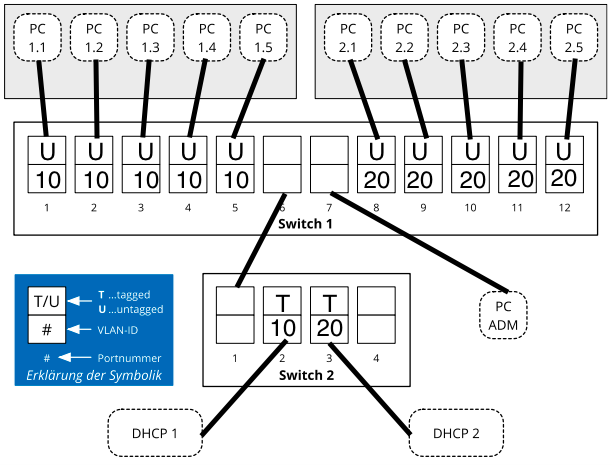
\includegraphics[width=0.75\textwidth]{./pics/Verkabelung}
	\end{center}
	Nein, ein Port kann nicht zeitgleich tagged und untagged sein, da es sonst einen Konflikt bei ankommenden Paketen geben würde: Einerseits müsste die VLAN-ID eingefügt werden (die noch nicht da war), andererseits müsste das Paket aufgrund fehlender VLAN-ID abgelehnt werden.

	\section*{Aufgabe 5}
	\begin{enumerate}[label=(\alph*)]
		\item Damit ein 1500-Byte-Frame korrekt ist, müssen alle 1500 Byte korrekt sein. Die Wahrscheinlichkeit dafür ist
		\begin{align}
			\mathbb{P}(\text{alle Frames korrekt}) &= (1-p)^{1500\cdot 8} \notag \\
			&= 0.9664 \notag
		\end{align}
		Die Wahrscheinlichkeit für einen Fehler liegt also bei 0.0336.
		\item Analog zu (a) gilt
		\begin{align}
			\mathbb{P}(\text{alle Frames korrekt}) &= (1-p)^{64\cdot 8} \notag \\
			&= 0.9985 \notag
		\end{align}
		Die Wahrscheinlichkeit für einen Fehler liegt also bei 0.15 \%.
	\end{enumerate}

	\section*{Aufgabe 6}
	\begin{center}
		\begin{tabular}{L{4cm}|L{5cm}|L{5cm}}
			 & \textbf{Ethernet} & \textbf{InfiniBand} \\
			 \hline
			 \textbf{Funktionsweise} & Datenpakete & RDMA (Remote Direct Memory Access), Daten werden zwischen den Speichern ausgetauscht; kein Overhead durch Netzwerkstack \\
			 \hline
			 \textbf{Datenraten} & 40 GbE (Kupfer/TP), 100 GbE (Glasfaser), 200/400GbE in Entwicklung & 2,5Gbps (SDR) bis 50 Gbps (HDR) je Kanal, Kanalbündelung bis zu 12 Kanälen: 600Gbps, 100 Gbps (NDR) und 250 Gbps (XDR) in Entw. \\
			 \hline
			 \textbf{Segmentlänge} & variiert sehr stark, von 1m bis 10+km Kupfer i.d.R bis 100m & Kupfer: bis 30m, Glasfaser bis 10km \\
			 \hline
			 \textbf{Latenzen} & gering & noch geringer \\
			 \hline
			 \textbf{Anwendungsgebiete} & Heimnetzwerk (LAN), Firmennetzwerk, Metro/Carrier Ethernet & Rechenzentren, Storage Area Networks, HPC, aber auch On-Premise Data Center \\
			 \hline
			 \textbf{Kompatibilität} & Ethernet over InfiniBand & RDMA over Converged Enhanced Ethernet
		\end{tabular}
	\end{center}
	
\end{document}